\newpage

\section*{ \hfill OCLA Debug Subsystem}
\addcontentsline{toc}{section}{OCLA Debug Subsystem}


% \lipsum

\subsection*{\fontsize{14}{16}\selectfont The Generated OCLA IP Wrapper}
\addcontentsline{toc}{subsection}{The Generated OCLA IP Wrapper}

After the IP customization and generation step, a top wrapper plus all source file are made available to the user.\\ 
The generated top wrapper file for OCLA \ref{fig:ocla_wrpr} has two different clocks i.e., the sample clock and the AXI clock. The sample clock of the OCLA is to be connected with
the design being monitored and the AXI clock is to be connected to an AXI bus clock.\\ The signals of the design that are to be sampled are connected to the probes port of the OCLA and the user specified input triggers signals can be connected to the corresponding 
port in the top wrapper. \\For the OCLA configuration and to read the sampled data from the OCLA the AXI-lite slave interface can be connected to an AXI bus.      

\begin{figure}[h]\centering % Using \begin{figure*} makes the figure take up the entire width of the page
	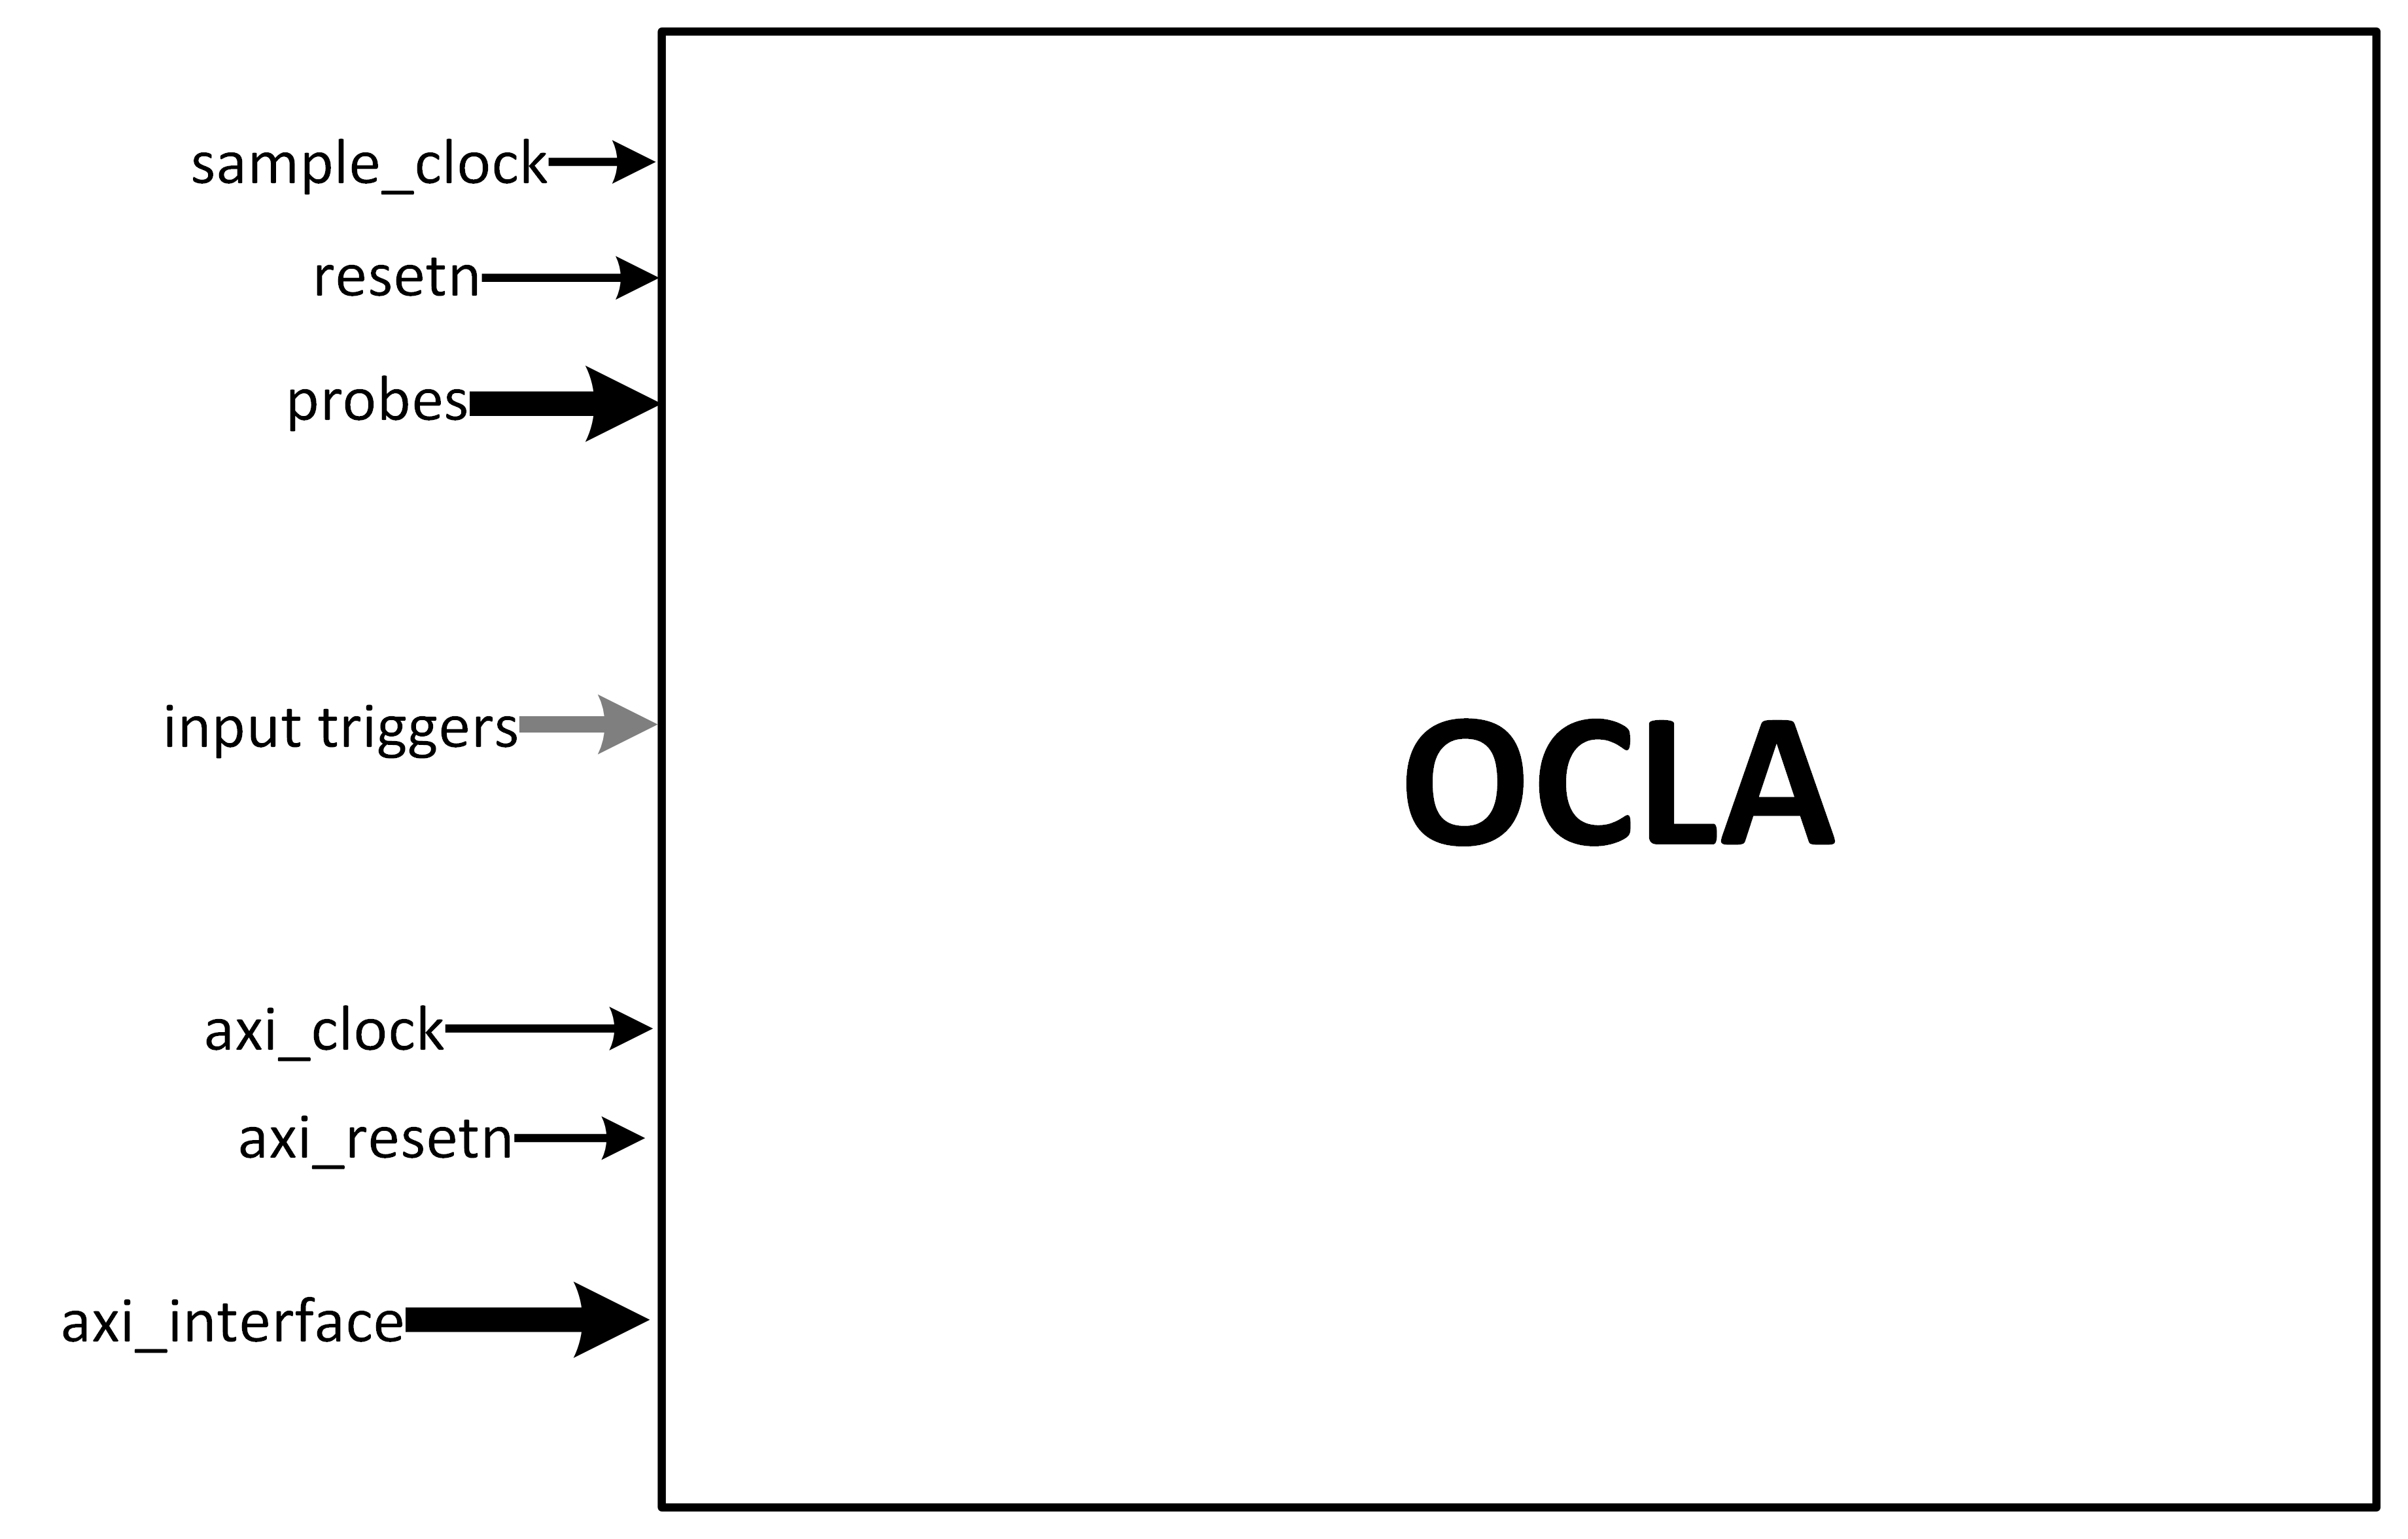
\includegraphics[width=.3\linewidth]{ocla_wrpr}
	\caption{\fontsize{8}{9}\selectfont OCLA TOP}
	\label{fig:ocla_wrpr}
\end{figure}
% \lipsum

\subsection*{\fontsize{14}{16}\selectfont OCLA Debug Subsystem}
\addcontentsline{toc}{subsection}{OCLA Debug Subsystem}
The OCLA top wrapper can be instantiated in a subsystem like the one shown in the figure \ref{fig:ocla_subsystem} for debugging purpose. \\In the debug
subsystem the OLCA IP core is integrated in between the AXI bus and the design being monitored.\\All the runtime OCLA configurations are controlled though JTAG interface.    

% \lipsum

\begin{figure}[h]\centering % Using \begin{figure*} makes the figure take up the entire width of the page
	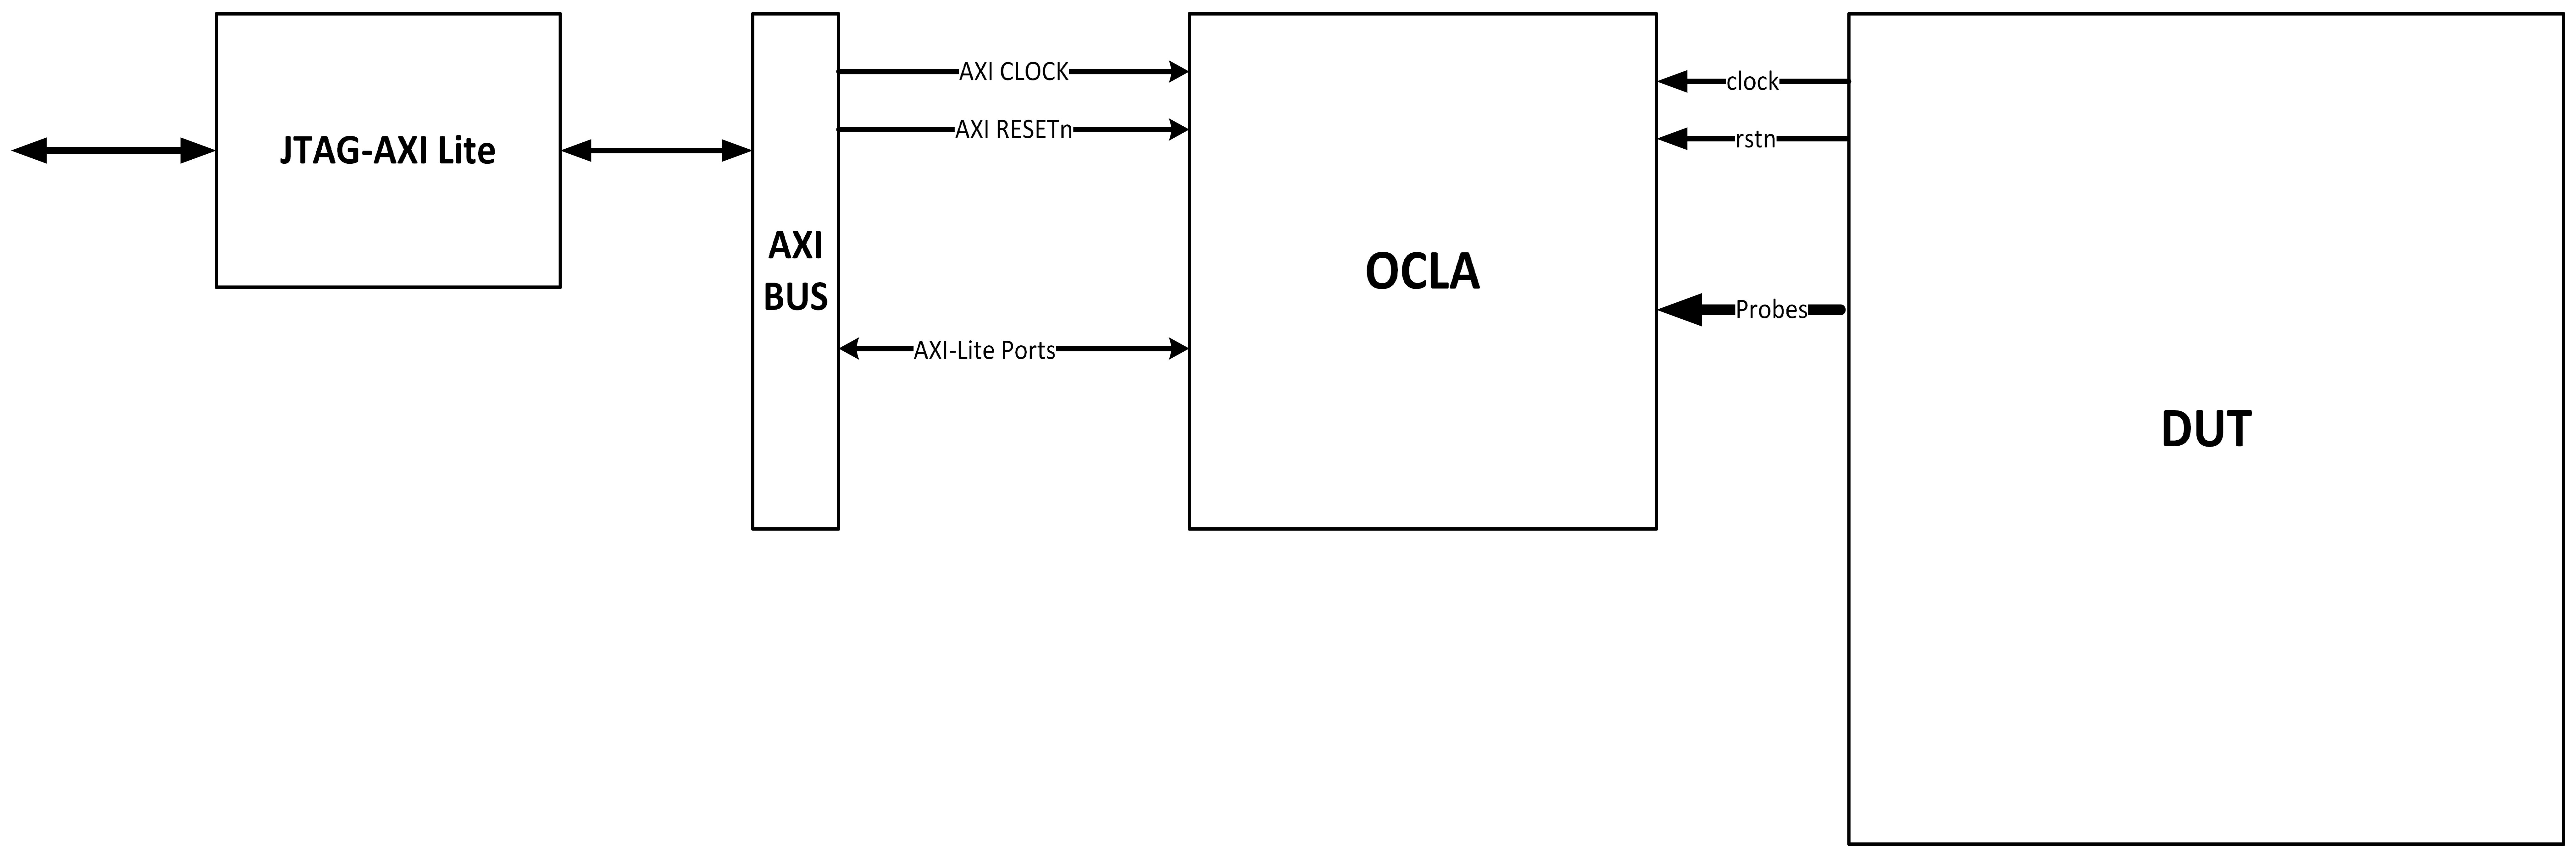
\includegraphics[width=\linewidth]{ocla_subsystem}
	\caption{\fontsize{8}{9}\selectfont OCLA Debug Subsystem}
	\label{fig:ocla_subsystem}
\end{figure}

% \lipsum

